





\chapter{Tag Clouds}
\label{sec:tagclouds}

Tags are used as simple means to describe a collection of resources by just giving names, called tags, to the resources in the corpus. Tag clouds are generated by collection of tags, and one of their first uses was for annotating pictures, as a part of Flickr\footnote{\url{http://www.flickr.com/}, accessed December, 2010} website in 2004~\cite{folksonomiesWeb2.0_2009}. Tags, created by different users, for a folksonomy, which is a flat user-generated classification of a collection of resources. Folksonomies are part of a new generation of tools for the retrieval, deployment, representation and production of information, commonly termed \textit{Web 2.0}. In Web 2.0 it is no longer just authors, web designers, journalists, or organizations who generate content - every user can do so via numerous online services and through various media, such as photos, videos or text. The heavy growth of user-generated content, a part of the so called \textit{information flood}, increases the demand for suitable methods and facilities for the storage and retrieval of said content. In order to meet those demands, collaborative information services have been developed, like social bookmarking, photo sharing and video sharing, where users index their own information resources with own customized tags. This indirect cooperation of users creates a folksonomy for each collaborative information services comprised of each individuals user's tags. Using this folksonomy, all users may then access the resources of the information service in question. \\ 

We give some basic concepts, used in this chapter:\\

\textit{Folksonomies} are flat, user-generated classifications. \\

\textit{Collaborative tagging} systems, also called \textit{social bookmarking systems}, are used to organize, browse and share personal collections of resources by introducing simple meta data about these resources~(fig.~\ref{collaborativeTagging}). \\

\textit{Tagging}, which is one of the defining characteristics of Web 2.0 services, allows users to collectively classify and find information. Tagging is manual (collaborative), done in social bookmarking applications, or automatically generated, e.g., based on frequency of term occurrence in collection of documents.\\

\textit{Tag clouds} are visual interfaces for \gls{IR} that provide a global contextual view of tags assigned to resources in the system~(fig.~\ref{fig:tagcloud}). \\


\textit{Web 2.0}. The context that houses collaborative information services is termed \textit{Web 2.0}. Web 2.0 spsans all activities and technical requirements that allow users of the World Wide Web to self-publish content, in the form of profiles, bookmarks, photos, videos, posts etc. and to make it accessible to other users, as well as to communicate with them~\cite{folksonomiesWeb2.0_2009}. \\


%TODO
%generate a tag cloud based on the contents in docmachine!!!!!!! replace the figure
%
% Opencloud
%
\begin{figure}[htbp]
	\centering
	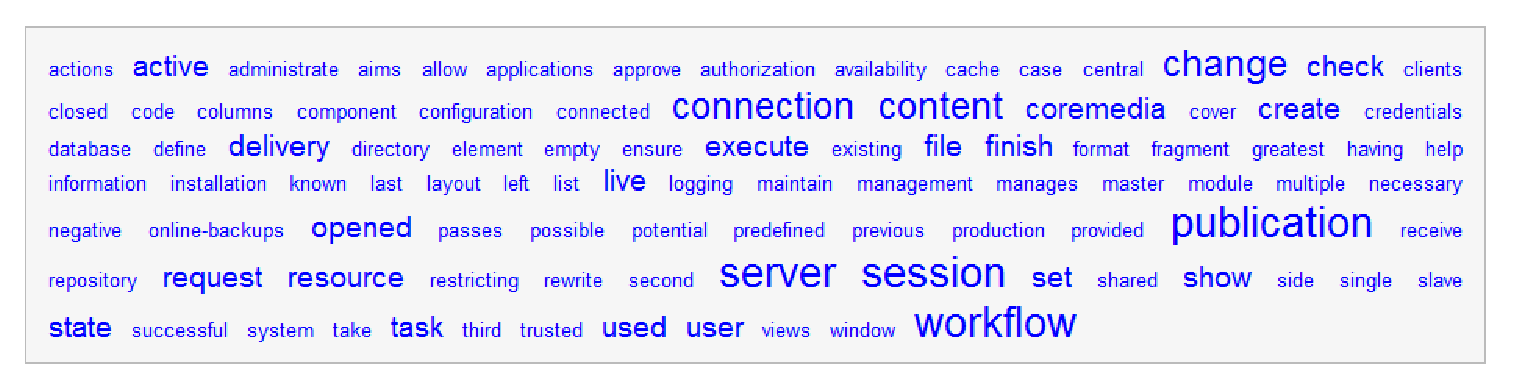
\includegraphics[width=\ScaleIfNeeded]{img/tagcloud} 
 % or [scale=0.5]
	\caption[A tag cloud.]{A tag cloud, where tags have been selected and visually weighted according to their frequency of use. \textbf{TODO:} change with a tag cloud from CM domain. }
	\label{fig:tagcloud}
\end{figure}

\section{Introduction}

Types of tag clouds: \\
\begin{itemize}
\item Tag clouds generated over partial lists, such as search results. The size of tags depends on the frequency of occurrence of the corresponding terms, measure for example using $tf-idf$  measure~(section~\ref{lsa:tf-idf-section}).\\
\item \textit{Collaborative tag clouds}, where tag frequencies (and size) are generated over all documents in the set.
text clouds, where clouds present main concepts, the size of tags measures importance, frequency of occurrence, etc. \\
\item \textit{ Categorical tag clouds}, where the size of tags reflects the size of corresponding category. \\
\end{itemize}
Tag clouds enhance the visualization of data. According to Smith~\cite{tagging2008} and Peters~\cite{folksonomiesWeb2.0_2009} tagging has the following main application areas: \\
\begin{itemize}
\item \textit{Information retrieval}, e.g. in the online services Last.fm\footnote{\url{http://www.lastfm.de/}, accessed December, 2010} or Engineering village\footnote{\url{http://www.engineeringvillage.org/}, accessed December, 2010}, where tag clouds enhance \gls{IR}, and are used to retrieve resources. Here are also included tag clouds used in e-commerce services, such as Amazon~\footnote{\url{http://www.amazon.com/gp/tagging/cloud/}, accessed December, 2010}.

\item \textit{Online libraries} use tag clouds to present book content in the form of main concepts, for example in Library Thing\footnote{\url{http://www.librarything.com/}, accessed December, 2010}, or to save bookmarks to electronic books, as in  . And these are just two examples out of many more. \\

\item \textit{Social bookmarking}. Delicious\footnote{\url{http://www.delicious.com/}, accessed December, 2010} offers tagging for sharing bookmarks to online resources, and the infamous Facebook\footnote{\url{http://www.facebook.com/}, accessed December, 2010}  uses tagging for sharing photos, videos or music. \\

\item As a part of \textit{games with a purpose}, or \textit{GWAP}\footnote{\url{http://www.gwap.com/}, accessed December, 2010}, where tagging is used for improving computer programs, such as programs performing image recognition tasks, for tagging audio or image files. \\ 
\end{itemize}

As tags and tag clouds are heavily used in collaborative tagging, we give an example for tag cloud use in the context of social bookmarking software~(fig.~\ref{collaborativeTagging}). In this application users have the roles of both content creators and content consumers. As consumers, they can use tag clouds for retrieval of resources, and visualization. In fig.~\ref{collaborativeTagging}, the tag cloud contains the most commonly occurring tags in the system, and tag bookmarks contain for a given tag $t$, a list of the most recently posted URLs annotated with $t$.  \\  

% wcc graphically presented simplified
\begin{figure}
	\centering
	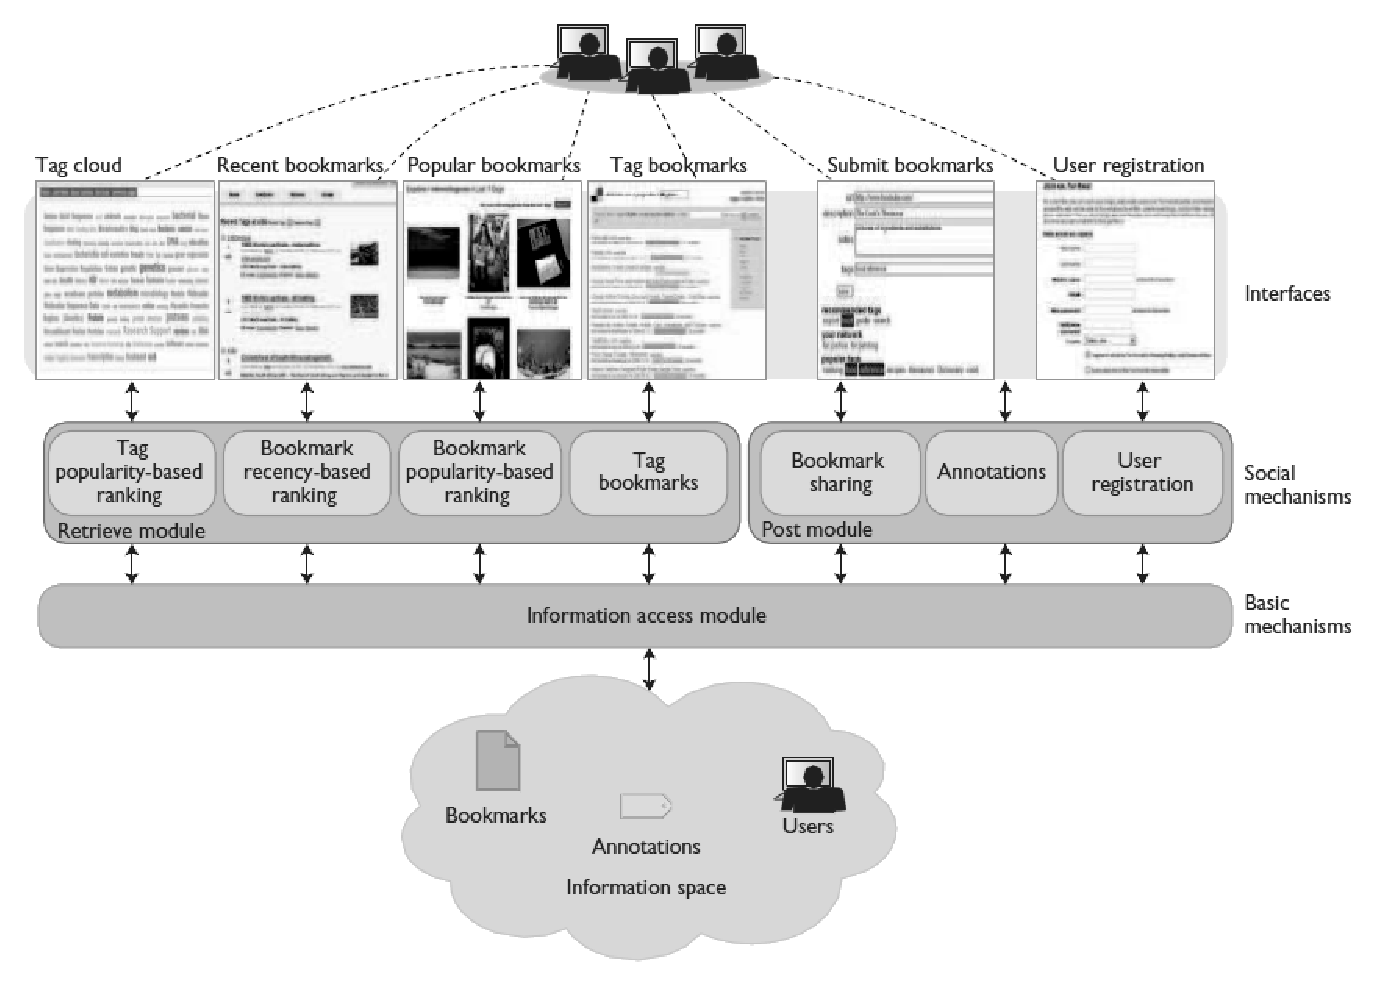
\includegraphics[scale=0.6]{img/collaborativeTagging} 
	\caption[Tag clouds in collaborative information services]
           {Tag clouds in applications for collaborative information services. Source: Heymann, Koutrika, Garcia-Molina(2007, ~\cite{tagcloud_spam2007})}
\label{collaborativeTagging}
\end{figure}

Using tagging in social bookmarking software has definite advantages. The extensive amount of people involved in the process of resource tagging can overcome to some extent the flood of information, generated on a daily basis by users. With respect to social bookmarking, Clay Shirky\footnote{\url{http://shirky.com/writings/ontology_overrated.html}, accessed December, 2010}, a professor at New York University, says: \textit{"The only group that can categorize everything is everybody."}. However social tagging has certain drawbacks. There is criticism about the quality of tagging, as it is usually done by laymen, and privacy issues arise, concerning the content generated by users~\cite{folksonomiesWeb2.0_2009}. \\




Tag clouds are visualization means extensively used in Internet. The come in three flavors: \\
\begin{itemize}
\item  $tf-idf$ clouds, generated using the frequency of occurrence of tags in a document, or a set of documents $D' \subset D$, where $D$ is the whole document collection;  
\item $collaborative$ clouds,  generated over the frequency of occurrence of tags in the whole collection $D$;
\item $categorical$ $tag$ $clouds$ in which tags represent categories. The size of their tags reflects the size of the categories which they represent.
\end{itemize}





\section{Tag clouds generation}
\textit{Tagging} is the activity of associating one or more key words or phrases to a resource. A tag is a label or a note that makes it easier for users to find online documents. Tags in this sense help to organize resources. Very popular colaborative tagging services are offered by Flickr\footnote{\url{http://www.flickr.com/}, accessed December, 2010} for images, Delicious\footnote{\url{http://www.delicious.com/}, accessed December, 2010} for web links, or Facebook\footnote{\url{http://www.facebook.com/}, accessed December, 2010} for social tagging. The users themselves annotate resources when using social tagging services. As a result, a tagspace is produced that can be efficiently searched. However, there still exist problems with polysemie and synonymy, as alredy discussed in Chapter~\ref{sec:lsa}. Another problem of tagging is when several users annotate the same resource in a different way. In order to increase the quality of retrieval in search engines, and avoid inconsistencies during user tagging, automatic tagging is implemented. Is is used mainly for annotation of news and blogs, in order offer to recommend to users suitable key words. It uses three terms from each message, that occur most often, based on $tf-idf$ measure~(section~\ref{lsa:tf-idf-section}).   \\

In principle, the font size of a tag in a tag cloud is determined by its frequency of occurrence. For a word cloud of categories like weblogs, the frequency of use for example, corresponds to the number of weblog entries that are assigned to a category. For small frequencies it's sufficient to indicate directly for any number from one to a maximum font size. For larger values, a scaling should be made. In a linear normalization, the weight $t_{i}$ of a tag is mapped to a size scale of $1$ through $f$, where $t_{min}$ and $t_{max}$ are specifying the range of available weights. \\
\begin{equation}
f_{i} = \lceil {\frac{f_{max} . (t_{i} - t_{min}}{t_{max} - t_{min})} }\rceil \mbox{ for }  t_{i} > t_{min}; \mbox{ else }  f_{i} = 1
\end{equation}

where $f_{i}$ is the displayed font-size, $f_{max}$ is the maximum font-size, $t_{i}$ is the count of tag $t$, and $t_{min}$, $t_{max}$ - the minimum and maximum count of term $t$. \\

Implementations of tag clouds also include text parsing and filtering out unhelpful tags such as common words, numbers, and punctuation. \\

\subsection{Tag cloud layout}

\begin{itemize}
\item Sequential layout, with either a horizontal or vertical arrangement of tags, sorted
alphabetically or by some other criteria (e.g., popularity, chronology, etc.).

\item Circular layout, with the most popular tags in the center and tags with decreasing
popularities towards the borders (or vice versa).
 
\item Clustered layout, in which the distance between tags follows a certain clustering
criteria (e.g., semantic relatedness) and related tags are positioned in close
proximity [3, 6].
\end{itemize}

The traditional tag cloud layout is alphabetical. \\
Tag clouds provide an aggregate of tag-usage statistics. They are typically sent as in-line HTML to browsers. \\
Since the font size of a displayed tag is usually used to show the relative importance or frequency of the tag, a typical tag cloud contains large and small text interspersed. \\

\section{Existing implementations}
In this work, we construct a semantic space over a set of documents using \gls{LSA}~(Chapter \ref{sec:lsa}), and use a tag cloud to visualize the main concepts in search results, retrieved from this space. Similar implementations of tag clouds exist, used to enhance \gls{IR} tasks. We give  examples of such applications below. \\

\textbf{Yippy}\footnote{\url{http://cloud.yippy.com/}, accessed Dezember, 2010} is a tool that visualizes topics based on search queries as a tag cloud, previously known as Clusty. Created by Vivisimo\footnote{\url{http://vivisimo.com/}, accessed Dezember, 2010}, it offers classification of search results. \\

\textbf{Google}\footnote{\url{http://www.google.com/}, accessed December, 2010} has developed their "Wonder wheel" search visualization tool, in order to display search results as a categorical tag cloud. The tags in Google's Wonder wheel represent categories in the set of search result documents. \\ 

\textbf{Opinion Crawl}\footnote{\url{http://www.opinioncrawl.com/}, accessed December, 2010} - web sentiment analysis application. It generates a concept cloud from daily scanned blogs, web site articles, and is developed at Semantic Engines LLC.\\

\textbf{SenseBot Search Results} is another tool from Semantic Engines LLC. It is a plugin for Mozilla Firefox browser that generates a tag cloud of the main concepts returned as search results from Google, included as a part of the SenseBot semantic search engine\footnote{\url{http://www.sensebot.net/}, accessed December, 2010}.\\

These are just a few examples of tag cloud usage which we present, as they are similar to the implementation purpose of the tag cloud developed in this work.  \\

\section{Conclusion}
In this chapter we presented tag clouds as visualization interfaces for enhancing \gls{IR} services, and discussed the use of tag clouds in the context of social bookmarking applications, and commercial retrieval systems. In the next chapter, we give the tag cloud implementation we developed as a part this work, and its function as a part of an \gls{IR} process. \\

